%% Chong Xing <cxing@ku.edu>
%% Paul Johnson <pauljohn@ku.edu>
%% 20190111
%% The path diagram for semexample/R/Ex-05-SEM/sem-02

%% standalone class for individual image to be included in a document
%% border=pt controls the whitespace padding around the diagram
\documentclass[border=15pt]{standalone}
\usepackage{tikz}
\usetikzlibrary{shapes}

\begin{document}

%% ">=latex" sets the arrow head style
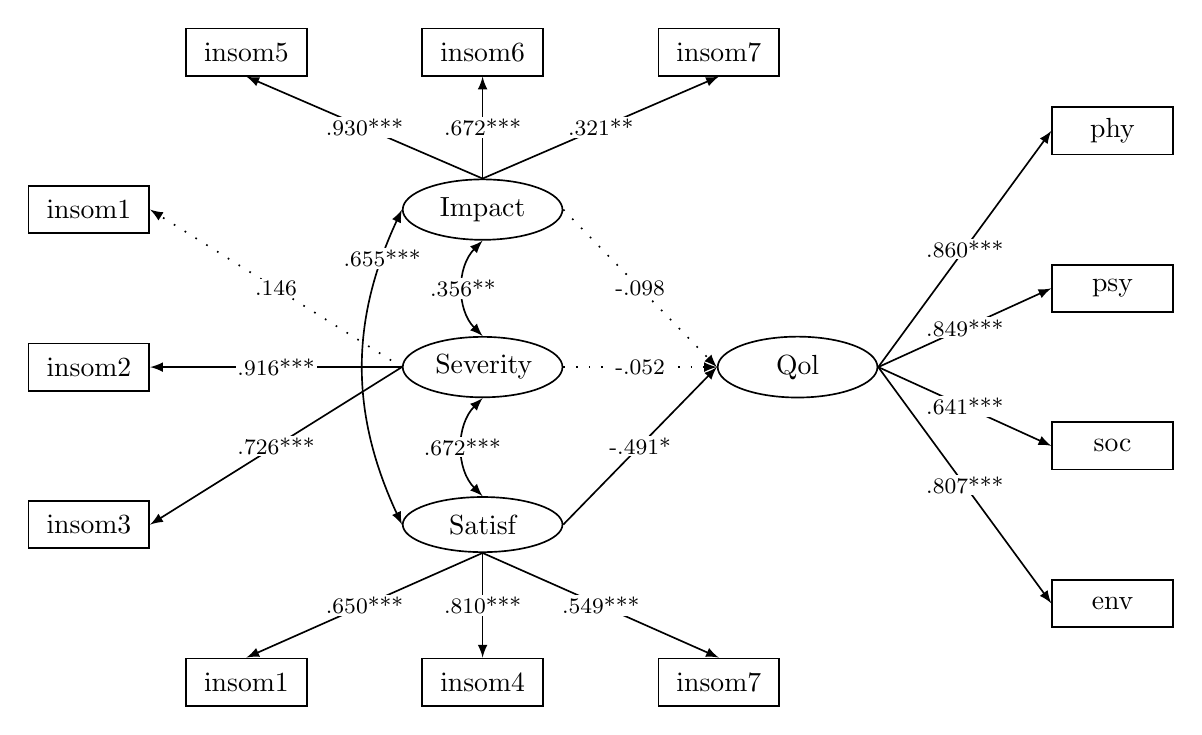
\begin{tikzpicture}[>=latex, semithick];

\node (exogenous1)  at (0, 2)  [draw, ellipse, align=center, text width=1.2cm, minimum height=0.7cm] {Impact};
\node (exogenous2)  at (0, 0)  [draw, ellipse, align=center, text width=1.2cm, minimum height=0.7cm] {Severity};
\node (exogenous3)  at (0, -2) [draw, ellipse, align=center, text width=1.2cm, minimum height=0.7cm] {Satisf};
\node (endogenous1) at (4, 0)  [draw, ellipse, align=center, text width=1.2cm, minimum height=0.7cm] {Qol};

\node (indicator1) at (-3, 4) [draw, text width=1.3cm, align=center, minimum height=0.6cm] {insom5};
\node (indicator2) at (0, 4)  [draw, text width=1.3cm, align=center, minimum height=0.6cm] {insom6};
\node (indicator3) at (3, 4)  [draw, text width=1.3cm, align=center, minimum height=0.6cm] {insom7};

\node (indicator4) at (-5, 2)  [draw, text width=1.3cm, align=center, minimum height=0.6cm] {insom1};
\node (indicator5) at (-5, 0)  [draw, text width=1.3cm, align=center, minimum height=0.6cm] {insom2};
\node (indicator6) at (-5, -2) [draw, text width=1.3cm, align=center, minimum height=0.6cm] {insom3};

\node (indicator7) at (-3, -4) [draw, text width=1.3cm, align=center, minimum height=0.6cm] {insom1};
\node (indicator8) at (0, -4)  [draw, text width=1.3cm, align=center, minimum height=0.6cm] {insom4};
\node (indicator9) at (3, -4)  [draw, text width=1.3cm, align=center, minimum height=0.6cm] {insom7};

\node (indicator10) at (8, 3)  [draw, text width=1.3cm, align=center, minimum height=0.6cm] {phy};
\node (indicator11) at (8, 1)  [draw, text width=1.3cm, align=center, minimum height=0.6cm] {psy};
\node (indicator12) at (8, -1) [draw, text width=1.3cm, align=center, minimum height=0.6cm] {soc};
\node (indicator13) at (8, -3) [draw, text width=1.3cm, align=center, minimum height=0.6cm] {env};

\path[->] (exogenous1.north) edge node[midway, fill=white, inner sep=0.7] {\footnotesize .930***} (indicator1.south);
\path[->] (exogenous1.north) edge node[midway, fill=white, inner sep=0.7] {\footnotesize .672***} (indicator2.south);
\path[->] (exogenous1.north) edge node[midway, fill=white, inner sep=0.7] {\footnotesize .321**}  (indicator3.south);

\path[->] (exogenous2.west) edge[loosely dotted] node[midway, fill=white, inner sep=0.7] {\footnotesize .146} (indicator4.east);
\path[->] (exogenous2.west) edge node[midway, fill=white, inner sep=0.7] {\footnotesize .916***} (indicator5.east);
\path[->] (exogenous2.west) edge node[midway, fill=white, inner sep=0.7] {\footnotesize .726***} (indicator6.east);

\path[->] (exogenous3.south) edge node[midway, fill=white, inner sep=0.7] {\footnotesize .650***} (indicator7.north);
\path[->] (exogenous3.south) edge node[midway, fill=white, inner sep=0.7] {\footnotesize .810***} (indicator8.north);
\path[->] (exogenous3.south) edge node[midway, fill=white, inner sep=0.7] {\footnotesize .549***} (indicator9.north);

\path[->] (endogenous1.east) edge node[midway, fill=white, inner sep=0.7] {\footnotesize .860***} (indicator10.west);
\path[->] (endogenous1.east) edge node[midway, fill=white, inner sep=0.7] {\footnotesize .849***} (indicator11.west);
\path[->] (endogenous1.east) edge node[midway, fill=white, inner sep=0.7] {\footnotesize .641***} (indicator12.west);
\path[->] (endogenous1.east) edge node[midway, fill=white, inner sep=0.7] {\footnotesize .807***} (indicator13.west);

\path[<->] (exogenous1.south) edge[bend right=45] node[midway, fill=white, inner sep=0.7]   {\footnotesize .356**}  (exogenous2.north);
\path[<->] (exogenous2.south) edge[bend right=45] node[midway, fill=white, inner sep=0.7]   {\footnotesize .672***} (exogenous3.north);
\path[<->] (exogenous1.west)  edge[bend right=25] node[pos=0.15, fill=white, inner sep=0.7] {\footnotesize .655***} (exogenous3.west);

\path[->] (exogenous1.east) edge[loosely dotted] node[midway, fill=white, inner sep=0.7] {\footnotesize -.098}  (endogenous1.west);
\path[->] (exogenous2.east) edge[loosely dotted] node[midway, fill=white, inner sep=0.7] {\footnotesize -.052}  (endogenous1.west);

\path[->] (exogenous3.east) edge node[midway, fill=white, inner sep=0.7] {\footnotesize -.491*} (endogenous1.west);

\end{tikzpicture}

\end{document}